%!TEX root = /Users/louis/Documents/PhD/Deliverables/ProgressReport/pr.tex
\section{Plan}
I have completed several of the activities outlined in the plan that was presented in my qualifying dissertation. However, I have experienced some difficulties when following that plan. A revised plan is presented in Section \ref{sub:revised_plan}. A discussion of the main goals of my research activities, and their relationship to the revised plan, is presented in Section \ref{sub:goals}.


\subsection{Existing Plan}
\label{sub:existing_plan}
Figure \ref{fig:old_plan} shows the research plan presented in my qualifying dissertation. I identified four activities to be completed before submitting my progress report. The status of those activities is as follows:

\begin{itemize}
	\item \textbf{Locate case studies}: Completed, as discussed in Section \ref{sub:examples}. However, locating example data took longer than I estimated in Figure \ref{fig:old_plan}. This caused ``Analyse case studies'' to start later than planned.
	\item \textbf{Analyse case studies}: Somewhat completed, as discussed in Section \ref{sub:analysis_of_existing_techniques}. In summary, I still need to use the example data to complete a review of existing co-evolution tools.
	\item \textbf{Co-evo and runtime evo lit review}: Completed, although I decided to focus more on model synchronisation literature, than runtime evolution literature as I found the former more interesting. The literature review lead to the elaboration of research aims discussed in Section \ref{sub:elaboration}.
	\item \textbf{Write progress report}: Completed.
\end{itemize}

In addition, I have made progress with the ``Plan metamodel evolution language'' activity, as discussed in Section~\ref{sub:development}. Although work on this activity was not due to start until February 2009, I proceeded while waiting for responses to requests for data for the ``Locate case studies'' activity.


\subsection{Revised Plan}
\label{sub:revised_plan}
Figure \ref{fig:revised_plan} shows my revised research plan. Originally, I had intended to begin planning a language for performing co-evolution in February 2009. However, I now feel that I am not yet able to identify requirements for the language. Consequently, I have introduced several new activities (``Plan stakeholder survey'', ``Analyse COPE'', ``Analyse Cicchetti's work'', ``Collaborate with Barber'', ``Collaborate with Sampson'') that will aid in defining requirements. These new activities are discussed in Section \ref{sub:goals}. Hence, the activities relating to developing the metamodel evolution language have been delayed. Furthermore, ``Develop metamodel evolution language'' and ``Evaluate user feedback'' now occupy one month (rather than six weeks) as I have already made some progress as discussed in Section \ref{sub:development}. Finally, Q4 2009 has also been updated to better reflect the progress made during that period.

% TODO: Evaluate user feedback seems unreasonable. Where will the feedback be obtained from?

When trying to follow the plan in Figure \ref{fig:old_plan}, I encountered some further difficulties. Firstly, some of the activities were too broad (such as ``Analyse case studies'' and ``Co-evo and runtime evo lit review'') and I had not identified clear goals, making progress hard to measure. Secondly, activities were unrealistically scheduled over the Christmas period.  In my revised plan (Figure \ref{fig:revised_plan}), I have decomposed large activities into several smaller activities. Goals for each of the activities are outlined in Section \ref{sub:goals}. In addition, I have not scheduled any activities during Christmas and Easter vacations.

\clearpage
\addtolength{\textwidth} {2in}
\addtolength{\topmargin} {1in}
\addtolength{\oddsidemargin} {-1.5in}
\begin{landscape}


\begin{figure}[ht]
  \begin{center}
    \leavevmode
    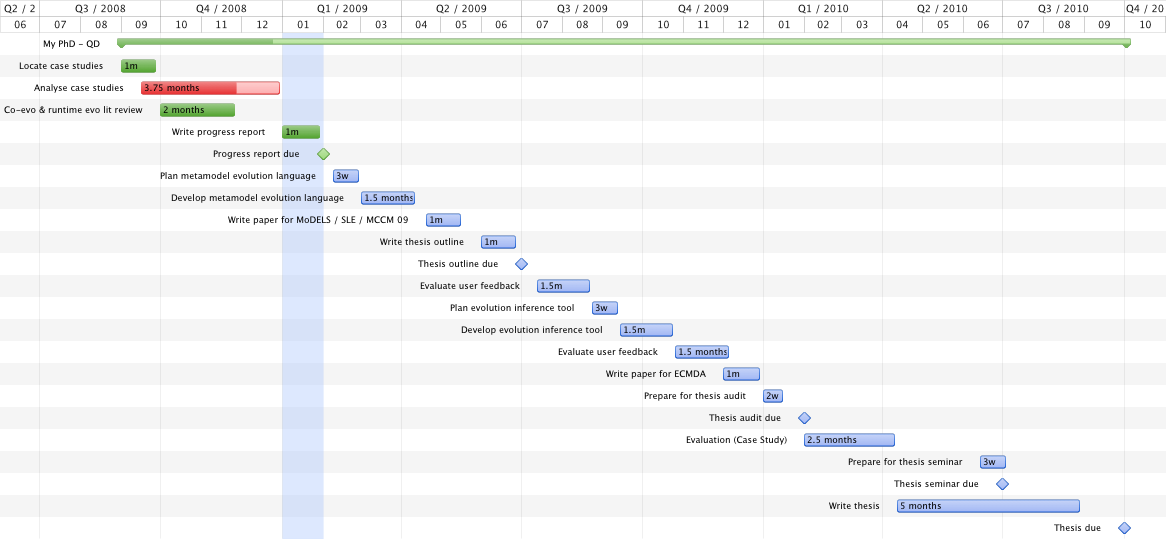
\includegraphics[scale=0.6]{old_plan.png}
  \end{center}
  \caption{Plan for my research, from my qualifying dissertation.}
  \label{fig:old_plan}
\end{figure}

\begin{figure}[ht]
  \begin{center}
    \leavevmode
    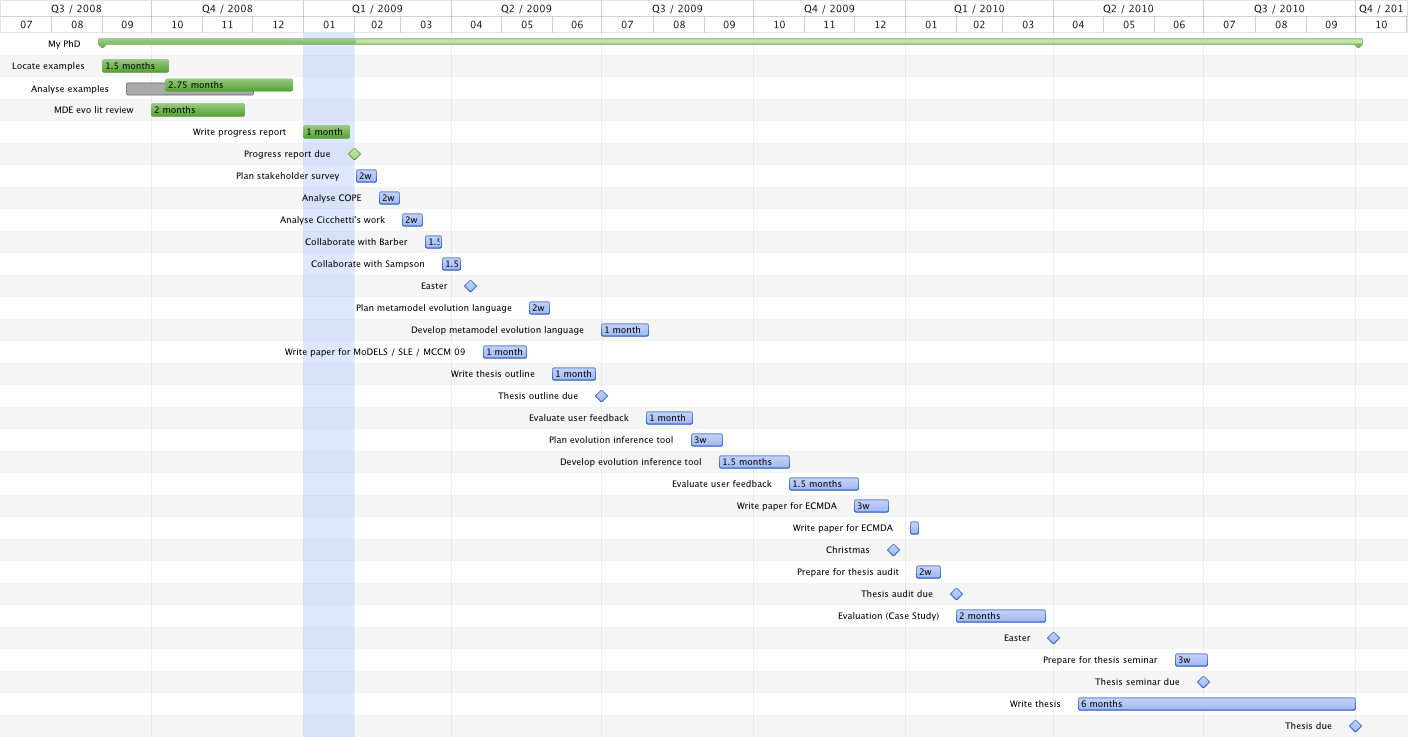
\includegraphics[scale=0.55]{revised_plan.png}
  \end{center}
  \caption{Revised plan for my research.}
  \label{fig:revised_plan}
\end{figure}

\end{landscape}
\addtolength{\oddsidemargin} {1.5in}
\addtolength{\topmargin} {-1in}
\addtolength{\textwidth} {-2in}

\subsection{Goals} % (fold)
\label{sub:goals}
Over the next three months, my primary goal is to determine requirements for a co-evolution language. The requirements will be identified by using examples of evolution from existing MDE projects to analyse existing co-evolution tools, by collaborating on incremental metamodel development with Barber and with Sampson, and by performing a survey of developers working on existing MDE projects.

Over the next year, I will use these requirements to develop structures and processes for co-evolutionary changes in the context of model-driven engineering. Specifically, I will develop a language for describing and executing co-evolution. Best practices for using the language will be identified by application to examples of evolution in existing MDE projects.

I anticipate that further structures and processes will be required to fulfil all of the identified requirements. Therefore, I will also develop an algorithm for automatically inferring migration strategies in response to metamodel changes.

My research will be evaluated using the Graphical Modelling Framework (GMF) \cite{gronback06gmf} as a case study. I will demonstrate that those problems occurring in GMF caused by evolutionary change can be managed using the structures and processes that I develop.

\subsubsection{February to June 2009}
I have identified several activities to be completed before I submit my thesis outline at the end of June 2009. Goals for each of these activities are now described. My thesis outline will contain goals for the activities to be performed between July 2009 and December 2009.

\paragraph{Plan stake-holder survey} % (fold)
\label{par:plan_stakeholder_survey}
No existing co-evolution research identifies requirements from developers working on MDE projects. By surveying developers working on existing MDE projects, I will ascertain data which will be used to derive requirements for my research. The survey will find answers to the following types of questions: Which tools are developers using for editing and versioning their models and metamodels? Are developers regularly introducing inconsistencies between their models and metamodels? Are developers performing co-evolution manually or using a tool? Which tools are being used for co-evolution?

I will survey developers working on MDE projects. I will seek participants from MODELPLEX, a European project focusing on using MDE to perform complex systems modelling, and conferences that discuss evolution in MDE (such as MCCM 2009). 

Before devising the survey, I will speak to members of the York Human Computer Interaction group, such as Chris Power and Paul Cairns. Both Power and Cairns have experience in developing surveys.

\subparagraph{Goals:} Devise and conduct a survey of developers working on existing MDE projects. Identify a process for devising an effective survey. Determine suitable questions, and use the answers to derive requirements for my thesis.

% paragraph plan_stakeholder_survey (end)


\paragraph{Analyse COPE and Cicchetti's work} % (fold)
\label{par:analyse_existing_work}
As discussed in Section \ref{sub:analysis_of_existing_techniques}, \cite{herrmannsdoerfer08cope,cicchetti08automating} both describe tools for performing co-evolution. By analysing both tools with data located from existing MDE projects, I will continue to identify areas in which these tools are effective, and ways in which they may be improved. The analysis will provide requirements for my research.

\subparagraph{Goals:} Use the example data discussed in Section \ref{sub:examples} to determine the effectiveness and shortcomings of existing tools for performing automated co-evolution. Use the findings to derive requirements for my research.

% paragraph analyse_existing_work (end)


\paragraph{Collaborate with Barber and with Sampson} % (fold)
\label{par:collaborate_with_barber_and_with_sampson}
I will continue to collaborate with Barber and with Sampson to iteratively and incrementally produce metamodels as discussed in Section \ref{par:collaborations}. Initially, I will collect a record of evolutionary changes made during the development of metamodels. If we encounter any evolutionary changes that inhibit development, I will be able to derive further requirements for my research.

\subparagraph{Goals:} Determine the extent to which the development of Barber's and Sampson's metamodels will aid my research. Observe and record any evolutionary changes made during the development. Obtain requirements from the data, and from Barber's and Sampson's experiences with MDE.

% paragraph collaborate_with_barber_and_with_sampson (end)


\paragraph{Plan metamodel evolution language} % (fold)
\label{par:plan_metamodel_evolution_language}
Before beginning any development, I will consolidate the results of previous activities to produce requirements for a co-evolution language. In addition, I will begin to prototype the language. The primary aim of the prototype will be for me to gain experience with any unfamiliar technologies.

\subparagraph{Goals:} Produce a list of requirements for a co-evolution language. Investigate any unfamiliar technologies that may aid in the development of the language.

% paragraph plan_metamodel_evolution_language (end)


\paragraph{Write paper for MoDELS / SLE / MCCM 2009} % (fold)
\label{par:write_paper_for_models_sle_mccm_2009}
The research conducted before July 2009 will yield publishable results. In particular, the collaboration with Barber will be used to generate a report describing our experiences with current MDE tools. We will be able to highlight the need for automated co-evolution tools and discuss why this need is not yet being fulfilled. The paper will strengthen the case for a claim that I will make in my thesis: that structures and processes for managing co-evolution are required in the context of model-driven engineering, and that existing tools are not satisfying this requirement.

\subparagraph{Goals:} Publish a paper at MoDELS 2009 (or co-located conferences). The paper will provide a basis for a chapter of my thesis.
% paragraph write_paper_for_models_sle_mccm_2009 (end)


\subsection{Summary}
In this report, software evolution and its impact on the maintainability of systems engineering using model-driven techniques have been introduced. Chapter \ref{sec:progress} restated and elaborated the aims of my research, presented the MDE projects that I will use to explore the effects of evolutionary change, discussed my analysis of existing tools for performing automated co-evolution; and presented the development status of a language for specifying and executing co-evolution.

Throughout this chapter, goals for developing my research have been presented, along with a timetable. The primary aim of my research will to be to produce requirements for, implement, and evaluate a language for specifying and executing co-evolution in the context of model-driven engineering.